\chapter{Geometrical Optics and Lenses}

\section{Fundamental Concepts}
\begin{itemize}
    \item \textbf{Geometrical Optics:} It is the study of light propagation in terms of rays, which travel in straight lines in homogeneous media. It is considered the limit where the wavelength tends to zero ($\lambda_0 \to 0$), ignoring effects such as diffraction and interference.
    \item \textbf{Point Source and Huygens' Principle:} A \textbf{point source} is an ideal emitter that radiates spherical waves. According to \textbf{Huygens' Principle}, any wavefront can be considered as a collection of countless point sources, where each emits its own spherical wavelets. The envelope of these wavelets forms the next wavefront.
    \item \textbf{Conjugate Points (S and P):} If rays originating from a point S converge to another point P after passing through an optical system, S and P are conjugate points. P is the \textbf{image} of S.
    \item \textbf{Real Image:} It is formed where light rays actually converge. It can be projected onto a screen.
    \item \textbf{Virtual Image:} It is formed where light rays appear to diverge. It cannot be projected onto a screen.
    \item \textbf{Optical Path Length (OPL):} In its generalized form, it is the integral of the refractive index along the path C: $OPL = \int_C n(s) ds$. For observation in a single homogeneous medium, it simplifies to $OPL = n \cdot d$. According to Fermat's Principle, light follows the path with the stationary OPL (minimum, maximum, or inflection).
\end{itemize}

\section{Refraction at Spherical Surfaces}

\begin{table}[h!]
\centering
\caption{Sign Convention for Spherical Refracting Surfaces and Thin Lenses (Light incident from the left)}
\begin{tabular}{ll}
\hline
\textbf{Quantity} & \textbf{Positive Sign (+)} \\ \hline
$s_o, f_o$ & to the left of V (vertex) \\
$x_o$ & to the left of $F_o$ (object focus) \\
$s_i, f_i$ & to the right of V (vertex) \\
$x_i$ & to the right of $F_i$ (image focus) \\
$R$ & if C (center of curvature) is to the right of V \\
$y_o, y_i$ & above the optical axis \\ \hline
\end{tabular}
\label{tab:signos_lentes}
\end{table}

\begin{table}[h!]
\centering
\caption{Meanings Associated with the Signs of Various Thin Lens and Spherical Interface Parameters}
\begin{tabular}{lcc}
\hline
\textbf{Quantity} & \multicolumn{1}{c}{\textbf{Sign (+) }} & \multicolumn{1}{c}{\textbf{Sign (-) }} \\ \hline
$s_o$ & Real object & Virtual object \\
$s_i$ & Real image & Virtual image \\
$f$ & Converging lens & Diverging lens \\
$y_o$ & Erect object & Inverted object \\
$y_i$ & Erect image & Inverted image \\
$M_T$ & Erect image & Inverted image \\ \hline
\end{tabular}
\label{tab:signos_significado}
\end{table}

In the paraxial approximation (rays close to the optical axis and with small angles), the relationship between the object distance ($s_o$) and the image distance ($s_i$) for a single spherical surface of radius $R$ separating two media with indices $n_1$ and $n_2$ is:

\begin{figure}[h]
    \centering
    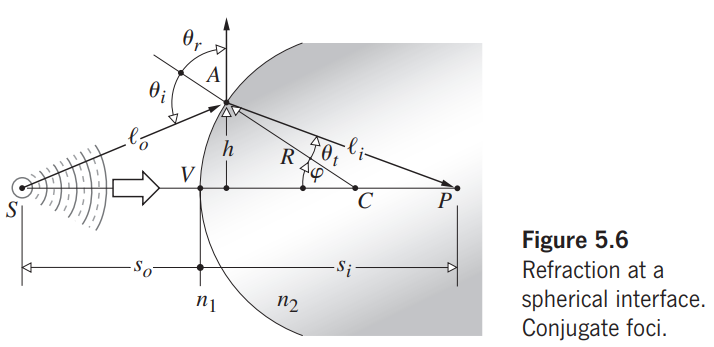
\includegraphics[width=0.7\linewidth]{1.png}
    \label{fig:placeholder}
\end{figure}

\vspace{0.5cm}
\noindent\fbox{%
\begin{minipage}{0.9\textwidth}
\begin{equation*}
    \frac{n_1}{s_o} + \frac{n_2}{s_i} = \frac{n_2 - n_1}{R}
\end{equation*}
\textbf{Hint:} This formula arises from applying Snell's Law in the paraxial approximation, where angles are small and we can use $\sin\theta \approx \theta$.
\end{minipage}
}
\vspace{0.5cm}

\begin{itemize}
    \item \textbf{Object Focal Length ($f_o$):} The object position for which the image is formed at infinity ($s_i = \infty$).
    $$ f_o = \frac{n_1 R}{n_2 - n_1} $$
    \item \textbf{Image Focal Length ($f_i$):} The image position when the object is at infinity ($s_o = \infty$).
    $$ f_i = \frac{n_2 R}{n_2 - n_1} $$
\end{itemize}

\section{Thin Lenses}
A thin lens is one whose thickness is negligible. Its behavior is described by two fundamental equations:

\begin{figure}[h]
    \centering
    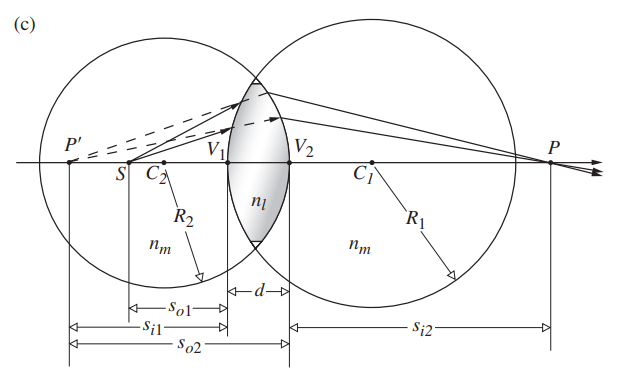
\includegraphics[width=0.55\linewidth]{spherical.png}
    \caption{A spherical lens}
    \label{fig:placeholder}
\end{figure}\\

\vspace{0.5cm}
\noindent\fbox{%
\begin{minipage}{0.9\textwidth}
\textbf{Lensmaker's Equation:} Relates the focal length ($f$) to the physical properties of the lens.
\begin{equation*}
    \frac{1}{f} = (n_l - 1) \left( \frac{1}{R_1} - \frac{1}{R_2} \right)
\end{equation*}
\textbf{Hint:} It is obtained by applying the refraction formula for a spherical surface to the two surfaces of the lens and assuming the thickness is zero.
\end{minipage}
}
\vspace{0.5cm}

\noindent\fbox{%
\begin{minipage}{0.9\textwidth}
\textbf{Gaussian Lens Equation:} Relates the positions of the object ($s_o$), the image ($s_i$), and the focus ($f$).
\begin{equation*}
    \frac{1}{s_o} + \frac{1}{s_i} = \frac{1}{f}
\end{equation*}
\textbf{Hint:} It is a simplification of the Lensmaker's Equation for practical use, note that it is a combination of the previous equations by applying transitivity.
\end{minipage}
}
\vspace{0.5cm}

\begin{itemize}
    \item \textbf{Converging Lenses (Positive):} They are thicker in the center. They have a positive focal length ($f > 0$) and converge parallel rays.
    \item \textbf{Diverging Lenses (Negative):} They are thinner in the center. They have a negative focal length ($f < 0$) and diverge parallel rays.
\end{itemize}

\vspace{1cm}

\subsubsection*{Images Formed by a Converging Lens (Convex)}
\begin{center}
\begin{tabular}{|l|llll|}
\hline
\multicolumn{1}{|c|}{\textbf{Object}} & \multicolumn{4}{c|}{\textbf{Image}} \\ \hline
\textbf{Position} & \textbf{Type} & \textbf{Position} & \textbf{Orientation} & \textbf{Relative Size} \\ \hline
$\infty > s_o > 2f$ & Real & $f < s_i < 2f$ & Inverted & Reduced \\
$s_o = 2f$ & Real & $s_i = 2f$ & Inverted & Same size \\
$f < s_o < 2f$ & Real & $\infty > s_i > 2f$ & Inverted & Magnified \\
$s_o = f$ & \multicolumn{4}{c|}{Image at $\pm \infty$} \\
$s_o < f$ & Virtual & $|s_i| > s_o$ & Erect & Magnified \\ \hline
\end{tabular}
\end{center}

\vspace{1cm}

\subsubsection*{Images Formed by a Diverging Lens (Concave)}
\begin{center}
\begin{tabular}{|l|llll|}
\hline
\multicolumn{1}{|c|}{\textbf{Object}} & \multicolumn{4}{c|}{\textbf{Image}} \\ \hline
\textbf{Position} & \textbf{Type} & \textbf{Position} & \textbf{Orientation} & \textbf{Relative Size} \\ \hline
Any position & Virtual & $|s_i| < |f|$, $s_o > |s_i|$ & Erect & Reduced \\ \hline
\end{tabular}
\end{center}

\section{Image Formation and Magnification}

\begin{figure}[h]
    \centering
    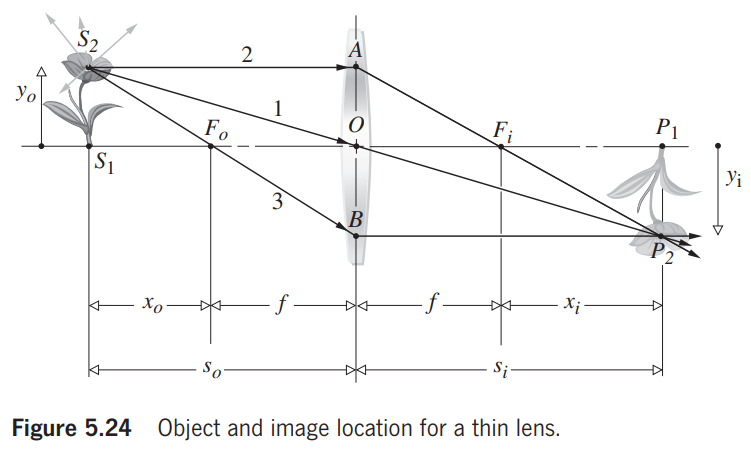
\includegraphics[width=0.75\linewidth]{diagram.png}
    \label{fig:placeholder}
\end{figure}

\begin{itemize}
    \item \textbf{Ray Tracing (Lenses):} The image of an object can be found graphically using three principal rays:
    \begin{enumerate}
        \item A ray passing through the optical center of the lens is not deviated.
        \item A ray parallel to the optical axis is refracted through the image focus ($F_i$).
        \item A ray passing through the object focus ($F_o$) is refracted parallel to the optical axis.
    \end{enumerate}
\end{itemize}

\noindent\fbox{%
\begin{minipage}{0.9\textwidth}
\textbf{Transverse Magnification ($M_T$):} It is the ratio of the image size ($y_i$) to the object size ($y_o$).
\begin{equation*}
    M_T = \frac{y_i}{y_o} = -\frac{s_i}{s_o}
\end{equation*}
\textbf{Hint:} It is derived from the similarity of triangles formed by the ray passing through the optical center. The negative sign indicates that a real image ($s_i > 0$) is inverted.
\end{minipage}
}
\vspace{0.5cm}

\noindent\fbox{%
\begin{minipage}{0.9\textwidth}
\textbf{Newtonian Formula:} Relates the distances from the foci.
\begin{equation*}
    x_o x_i = f^2
\end{equation*}
\textbf{Hint:} It is an alternative form of the Gaussian equation, useful when measuring from the foci instead of the lens center.
\end{minipage}
}

\section{Combination of Lenses}
The analysis of systems with multiple lenses is based on a simple principle: the image formed by the first lens becomes the \textbf{object} for the second lens, and so on. The image from the previous lens can be a real object (if it forms before the next lens) or a virtual object (if it would form after the next lens).

\subsection*{Lenses in Contact}
When two thin lenses are in contact ($d \to 0$), they behave as a single thin lens whose power is the sum of the individual powers.

\vspace{0.5cm}
\noindent\fbox{%
\begin{minipage}{0.9\textwidth}
\textbf{Effective Focal Length (Lenses in Contact):}
\begin{equation*}
    \frac{1}{f_{\text{eff}}} = \frac{1}{f_1} + \frac{1}{f_2}
\end{equation*}
\textbf{Hint:} This is the simplest form of combination. It is deduced by treating the image of $L_1$ as the object for $L_2$ and letting the separation $d$ tend to zero in the more general equations.
\end{minipage}
}
\vspace{0.5cm}

\subsection*{Separated Lenses}
When lenses are separated by a distance $d$, the system can no longer be described with a single focal length measured from a single point. Instead, two principal focal lengths are defined, measured from the outer lenses of the system.

\subsubsection*{Back Focal Length (b.f.l.)}
The \textbf{physical meaning} of the b.f.l. is that it indicates where the final focus will be formed for rays entering the system parallel (i.e., from an object at infinity). It is the distance from the vertex of the \textbf{last lens} to the image focal point of the entire system. It is crucial for knowing where to place a sensor or film.

\vspace{0.5cm}
\noindent\fbox{%
\begin{minipage}{0.9\textwidth}
\textbf{Back Focal Length Formula:}
\begin{equation*}
    \text{b.f.l.} = \frac{f_2(d - f_1)}{d - (f_1 + f_2)}
\end{equation*}
\textbf{Hint:} It is obtained by taking the limit as the initial object is at infinity ($s_{o1} \to \infty$) and calculating the position of the final image ($s_{i2}$) with respect to the second lens.
\end{minipage}
}
\vspace{0.5cm}

\subsubsection*{Front Focal Length (f.f.l.)}
The \textbf{physical meaning} of the f.f.l. is that it indicates where an object must be placed so that the rays exit the system parallel (i.e., so that the final image is at infinity). It is the distance from the vertex of the \textbf{first lens} to the object focal point of the entire system.

\vspace{0.5cm}
\noindent\fbox{%
\begin{minipage}{0.9\textwidth}
\textbf{Front Focal Length Formula:}
\begin{equation*}
    \text{f.f.l.} = \frac{f_1(d - f_2)}{d - (f_1 + f_2)}
\end{equation*}
\textbf{Hint:} It is obtained by imposing the condition that the final image is at infinity ($s_{i2} \to \infty$) and calculating the required position of the initial object ($s_{o1}$) with respect to the first lens.
\end{minipage}
}

\chapter{Stops and Mirrors}

\section{*Stops}
\begin{itemize}
    \item \textbf{Aperture Stop (A.S.):} The physical element that limits the amount of light reaching the image. It determines the brightness.
    \item \textbf{Field Stop (F.S.):} The element that limits the size of the object that can be seen. It determines the field of view.
    \item \textbf{Entrance Pupil:} The image of the A.S. as seen from the object space.
    \item \textbf{Exit Pupil:} The image of the A.S. as seen from the image space. This is where the eye should be placed.
\end{itemize}

\section{*Relative Aperture and f-number}
\noindent\fbox{%
\begin{minipage}{0.9\textwidth}
\textbf{f-number ($f/\#$):} Relates the focal length ($f$) and the diameter of the entrance pupil ($D$).
\begin{equation*}
    f/\# = \frac{f}{D}
\end{equation*}
\textbf{Hint:} It is a definition that relates the light-gathering capability (diameter D) with the magnification (focal length f). A small f-number implies a "fast" lens.
\end{minipage}
}

\section{Spherical Mirrors}
Unlike plane mirrors, spherical mirrors can focus light and form magnified or reduced images. They are governed by two fundamental equations in the paraxial approximation.

\begin{table}[h!]
\centering
\caption{Sign Convention for Spherical Mirrors}
\begin{tabular}{lcc}
\hline
\textbf{Quantity} & \multicolumn{1}{c}{\textbf{Sign (+) }} & \multicolumn{1}{c}{\textbf{Sign (-) }} \\ \hline
$s_o$ & Left of V, real object & Right of V, virtual object \\
$s_i$ & Left of V, real image & Right of V, virtual image \\
$f$ & Concave mirror & Convex mirror \\
$R$ & C to the right of V, convex & C to the left of V, concave \\
$y_o$ & Above axis, erect object & Below axis, inverted object \\
$y_i$ & Above axis, erect image & Below axis, inverted image \\ \hline
\end{tabular}
\label{tab:signos_espejos}
\end{table}

\vspace{0.5cm}
\noindent\fbox{%
\begin{minipage}{0.9\textwidth}
\textbf{Mirror Formula (in terms of R):} Relates the object ($s_o$) and image ($s_i$) distances with the radius of curvature ($R$) of the mirror.
\begin{equation*}
    \frac{1}{s_o} + \frac{1}{s_i} = -\frac{2}{R}
\end{equation*}
\textbf{Hint:} This is the main form of the equation, derived directly from the Law of Reflection and the geometry of triangles in the paraxial approximation.
\end{minipage}
}
\vspace{0.5cm}

\noindent\fbox{%
\begin{minipage}{0.9\textwidth}
\textbf{Focal Length ($f$):} It is defined in terms of the radius of curvature.
\begin{equation*}
    f = -\frac{R}{2}
\end{equation*}
\textbf{Hint:} For paraxial rays, the focus of a spherical mirror is located halfway to the center of curvature. The negative sign is a consequence of the sign convention (for a concave mirror, $R<0$, resulting in a positive focus, $f>0$).
\end{end{minipage}
}
\vspace{0.5cm}

By combining the two expressions above, we obtain the most common form of the mirror formula, which is identical to the thin lens equation:
$$ \frac{1}{s_o} + \frac{1}{s_i} = \frac{1}{f} $$

\begin{itemize}
    \item \textbf{Concave Mirrors:} They have $R < 0$, so their focal length is positive ($f > 0$). They behave analogously to converging lenses.
    \item \textbf{Convex Mirrors:} They have $R > 0$, so their focal length is negative ($f < 0$). They behave analogously to diverging lenses.
\end{itemize}

\subsection*{Image Characteristics for Spherical Mirrors}
The following table summarizes the properties of the image formed by concave and convex mirrors for a real object.

\vspace{0.5cm}
\subsubsection*{Concave Mirror}
\begin{center}
\begin{tabular}{|l|llll|}
\hline
\multicolumn{1}{|c|}{\textbf{Object}} & \multicolumn{4}{c|}{\textbf{Image}} \\ \hline
\textbf{Position} & \textbf{Type} & \textbf{Position} & \textbf{Orientation} & \textbf{Relative Size} \\ \hline
$\infty > s_o > 2f$ & Real & $f < s_i < 2f$ & Inverted & Reduced \\
$s_o = 2f$ & Real & $s_i = 2f$ & Inverted & Same size \\
$f < s_o < 2f$ & Real & $\infty > s_i > 2f$ & Inverted & Magnified \\
$s_o = f$ & \multicolumn{4}{c|}{Image at $\pm \infty$} \\
$s_o < f$ & Virtual & $|s_i| > s_o$ & Erect & Magnified \\ \hline
\end{tabular}
\end{center}

\vspace{1cm}

\subsubsection*{Convex Mirror}
\begin{center}
\begin{tabular}{|l|llll|}
\hline
\multicolumn{1}{|c|}{\textbf{Object}} & \multicolumn{4}{c|}{\textbf{Image}} \\ \hline
\textbf{Position} & \textbf{Type} & \textbf{Position} & \textbf{Orientation} & \textbf{Relative Size} \\ \hline
Any position & Virtual & $|s_i| < |f|$, $s_o > |s_i|$ & Erect & Reduced \\ \hline
\end{tabular}
\end{center}

\chapter{Prisms and Fiber Optics}

\section{Prisms}

\begin{itemize}
    \item \textbf{Dispersing Prisms:} They separate light by color due to the dependence of $n$ on $\lambda$.
\end{itemize}

\begin{figure}[h]
    \centering
    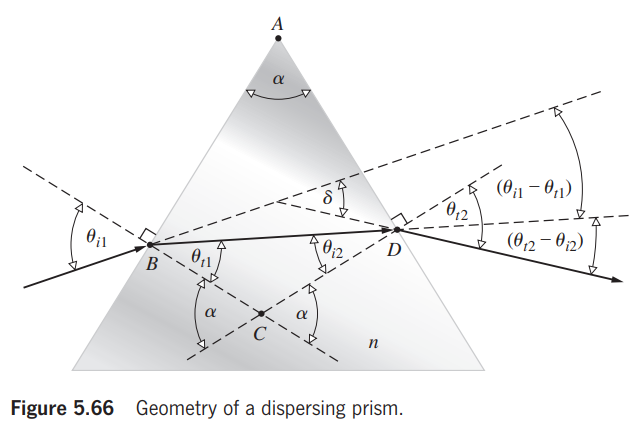
\includegraphics[width=0.55\linewidth]{prims disp.png}
    \label{fig:placeholder}
\end{figure}

\noindent\fbox{%
\begin{minipage}{0.9\textwidth}
\textbf{Refractive Index from Minimum Deviation ($\delta_m$):}
\begin{equation*}
    n = \frac{\sin\left(\frac{\delta_m + \alpha}{2}\right)}{\sin\left(\frac{\alpha}{2}\right)}
\end{equation*}
\textbf{Hint:} It is obtained by applying Snell's Law on both faces under the symmetric condition of minimum deviation, where the internal ray is parallel to the base.
\end{minipage}
}

\begin{itemize}
    \item \textbf{Reflecting Prisms:} They use total internal reflection to deviate light or invert images (e.g., Porro prism in binoculars).
\end{itemize}

\section{Fiber Optics}
They guide light through total internal reflection (TIR). They consist of a core ($n_f$) and a cladding ($n_c$), with $n_f > n_c$.

\noindent\fbox{%
\begin{minipage}{0.9\textwidth}
\textbf{Numerical Aperture (NA):} A measure of the fiber's ability to capture light.
\begin{equation*}
    \text{NA} = n_i \sin\theta_{\text{max}} = \sqrt{n_f^2 - n_c^2}
\end{equation*}
\textbf{Hint:} It comes from applying Snell's Law at the entrance face and the TIR condition ($ \sin\theta_c = n_c/n_f $) at the core-cladding interface.
\end{minipage}
}

\chapter{Optical Systems}
\section{The Human Eye and its Correction}
\begin{itemize}
    \item The eye forms a real and inverted image on the retina.
    \item \textbf{Myopia (Nearsightedness):} The eye is too convergent. It is corrected with a \textbf{diverging} (negative) lens.
    \item \textbf{Hyperopia (Farsightedness):} The eye is not convergent enough. It is corrected with a \textbf{converging} (positive) lens.
\end{itemize}

\noindent\fbox{%
\begin{minipage}{0.9\textwidth}
\textbf{Dioptric Power ($\mathcal{P}$):} The inverse of the focal length in meters.
\begin{equation*}
    \mathcal{P} \text{ [D]} = \frac{1}{f \text{ [m]}}
\end{equation*}
\textbf{Hint:} It is a definition of convenience. The power of lenses in contact adds up: $\mathcal{P} = \mathcal{P}_1 + \mathcal{P}_2$.
\end{minipage}
}

\section{Optical Instruments}
\noindent\fbox{%
\begin{minipage}{0.9\textwidth}
\textbf{Angular Magnification (Magnifier, image at $\infty$):}
\begin{equation*}
    MP = \frac{d_o}{f} \approx \frac{25 \text{ cm}}{f}
\end{equation*}
\textbf{Hint:} Compares the angle subtended by the virtual image with the angle subtended by the object at the near point ($d_o \approx 25$ cm).
\end{minipage}
}
\vspace{0.5cm}

\noindent\fbox{%
\begin{minipage}{0.9\textwidth}
\textbf{Angular Magnification (Microscope):}
\begin{equation*}
    MP = M_{To} M_{Ae} = \left(-\frac{L}{f_o}\right)\left(\frac{d_o}{f_e}\right)
\end{equation*}
\textbf{Hint:} It is the product of the linear magnification of the objective ($M_{To}$) and the angular magnification of the eyepiece ($M_{Ae}$). $L$ is the tube length ($\approx 160$ mm).
\end{minipage}
}
\vspace{0.5cm}

\noindent\fbox{%
\begin{minipage}{0.9\textwidth}
\textbf{Angular Magnification (Microscope):}
\begin{equation*}
    MP = M_{To} M_{Ae} = \left(-\frac{L}{f_o}\right)\left(\frac{d_o}{f_e}\right)
\end{equation*}
\textbf{Hint:} It is the product of the linear magnification of the objective ($M_{To}$) and the angular magnification of the eyepiece ($M_{Ae}$). $L$ is the tube length ($\approx 160$ mm).
\end{minipage}
}
\vspace{0.5cm}

\noindent\fbox{%
\begin{minipage}{0.9\textwidth}
\textbf{Angular Magnification (Telescope):}
\begin{equation*}
    MP = -\frac{f_o}{f_e}
\end{equation*}
\textbf{Hint:} It is the ratio of the subtended angles, which by similarity of triangles becomes the ratio of the focal lengths of the objective and the eyepiece.
\end{minipage}
}

\chapter{Thick Lenses}
Unlike a thin lens, a \textbf{thick lens} is one whose thickness is not negligible. To analyze these systems accurately, \textbf{analytical ray tracing} and its elegant formulation, the \textbf{matrix method}, are used.

\section{The Transfer Matrix Method}
The central idea is to model the path of a paraxial ray through an optical system using matrix operations. Each ray is represented by a vector and each element or space in the system by a matrix.

\begin{enumerate}
    \item \textbf{Ray Vector ($r$):} Describes the state of a ray by its height ($y$) and its weighted angle ($n\alpha$) at a point on the axis.
    \item \textbf{Operation Matrices:} They are applied to the ray vector to transform it. The two basic operations are:
    \begin{itemize}
        \item \textbf{Refraction ($\mathfrak{R}$):} The change in the ray's direction at an interface.
        \item \textbf{Translation ($\mathfrak{T}$):} The straight-line advance of the ray through a medium.
    \end{itemize}
\end{enumerate}

\vspace{0.5cm}
\noindent\fbox{%
\begin{minipage}{0.9\textwidth}
\textbf{Ray Vector ($r$):} Describes the height ($y$) and angle ($\alpha$) of a ray at a given point.
\begin{equation*}
    r = \begin{bmatrix} n\alpha \\ y \end{bmatrix}
\end{equation*}
\textbf{Hint:} This vector contains all the necessary information for a paraxial ray. The weighted angle ($n\alpha$) is used because it is modified simply in refraction and is conserved in translation.
\end{minipage}
}
\vspace{0.5cm}

\noindent\fbox{%
\begin{minipage}{0.9\textwidth}
\textbf{Refraction Matrix ($\mathfrak{R}$):} Models the change in the ray's direction as it passes through a surface of power $\mathcal{D}$.
\begin{equation*}
    \mathfrak{R} = \begin{bmatrix} 1 & -\mathcal{D} \\ 0 & 1 \end{bmatrix} \quad \text{where} \quad \mathcal{D} = \frac{n_t - n_i}{R}
\end{equation*}
\textbf{Hint:} This matrix only affects the ray's angle ($n\alpha$), not its height. The element $-\mathcal{D}$ represents the "strength" of the surface to bend light.
\end{minipage}
}
\vspace{0.5cm}

\noindent\fbox{%
\begin{minipage}{0.9\textwidth}
\textbf{Translation Matrix ($\mathfrak{T}$):} Models the straight-line travel of the ray over a distance $d$ in a medium of index $n$.
\begin{equation*}
    \mathfrak{T} = \begin{bmatrix} 1 & 0 \\ d/n & 1 \end{bmatrix}
\end{equation*}
\textbf{Hint:} This matrix only affects the ray's height ($y$), not its angle. The term $d/n$ represents the change in height due to propagation.
\end{minipage}
}
\vspace{0.5cm}

\section{The System Matrix and Cardinal Points}
To obtain the total effect of a thick lens, the matrices for each operation are multiplied in the \textbf{reverse} order to which the light encounters them. For a lens of thickness $d_l$ and index $n_l$:
$$ \mathcal{A} = \mathfrak{R}_2 \mathfrak{T}_{21} \mathfrak{R}_1 $$
This \textbf{System Matrix ($\mathcal{A}$)} encapsulates all the properties of the lens. Most powerfully, its elements are directly related to the \textbf{cardinal points}, which are the reference points that define any optical system.

\vspace{0.5cm}
\noindent\fbox{%
\begin{minipage}{0.9\textwidth}
\textbf{System Matrix ($\mathcal{A}$) for a Thick Lens:}
\begin{equation*}
\mathcal{A} = \begin{bmatrix} 1-\frac{\mathcal{D}_2 d_l}{n_l} & -\mathcal{D}_1-\mathcal{D}_2+\frac{\mathcal{D}_1 \mathcal{D}_2 d_l}{n_l} \\ \frac{d_l}{n_l} & 1-\frac{\mathcal{D}_1 d_l}{n_l} \end{bmatrix} = \begin{bmatrix} a_{11} & a_{12} \\ a_{21} & a_{22} \end{bmatrix}
\end{equation*}
\textbf{Hint:} The determinant of this matrix is always 1 ($|\mathcal{A}|=1$).
\end{minipage}
}
\vspace{0.5cm}

The cardinal points (focal points, principal planes, and nodal points) can be calculated directly from the elements of $\mathcal{A}$.

\begin{figure}[h]
    \centering
    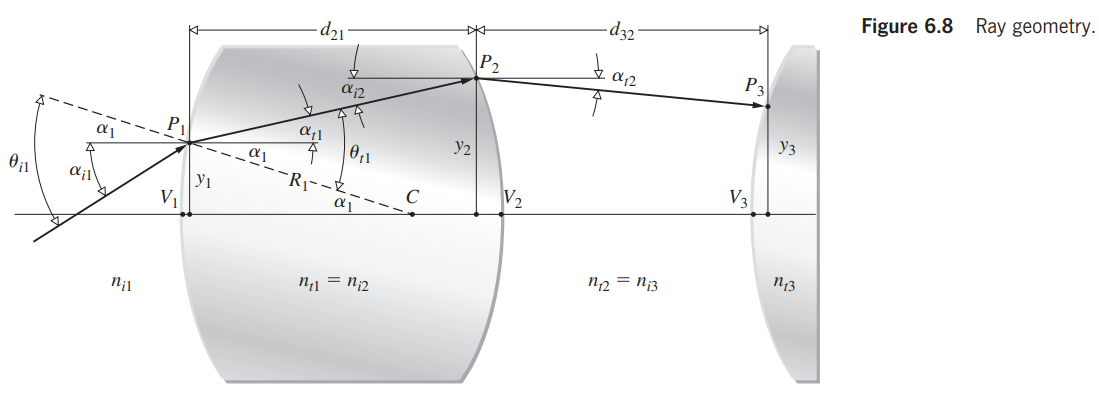
\includegraphics[width=0.85\linewidth]{rayt.png}
    \caption{Cardinal points and ray tracing in a thick lens.}
    \label{fig:placeholder}
\end{figure}

\begin{itemize}
    \item \textbf{Focal Points ($F_o, F_i$):} Define where rays focus or appear to originate from.
    \item \textbf{Principal Planes ($H_1, H_2$):} Are the theoretical planes where all refraction occurs. The focal length is measured from them.
    \item \textbf{Nodal Points ($N_1, N_2$):} A ray directed at $N_1$ emerges from $N_2$ with the same direction. In air, they coincide with the principal planes.
\end{itemize}

\noindent\fbox{%
\begin{minipage}{0.9\textwidth}
\textbf{Effective Focal Length ($f$):} The total power of the lens ($1/f$) is contained in the element $a_{12}$.
\begin{equation*}
    \frac{1}{f} = -a_{12}
\end{equation*}
\textbf{Hint:} This element represents the converging/diverging capability of the entire system.
\end{minipage}
}
\vspace{0.5cm}

\noindent\fbox{%
\begin{minipage}{0.9\textwidth}
\textbf{Position of the Principal Planes ($h_1, h_2$):} They are calculated from the lens vertices ($V_1, V_2$).
\begin{align*}
    h_1 &= \overline{V_1 H_1} = \frac{1-a_{11}}{-a_{12}} \\
    h_2 &= \overline{V_2 H_2} = \frac{a_{22}-1}{-a_{12}}
\end{align*}
\textbf{Hint:} These formulas locate the theoretical planes of refraction. A positive value means the plane is to the right of the vertex.
\end{minipage}
}
\vspace{0.5cm}

\section{Using Thick Lenses: Equations and Ray Tracing}
Once the effective focal length ($f$) and the position of the principal planes ($H_1, H_2$) are known, the analysis of a thick lens becomes very similar to that of a thin lens.

\begin{itemize}
    \item \textbf{Graphical Ray Tracing:} The same three principal rays are used, but refraction occurs at the planes $H_1$ and $H_2$, not at the center of the lens.
    \item \textbf{Lens Equations:} The Gaussian and Newtonian formulas are valid if the distances are measured from the principal planes.
\end{itemize}

\noindent\fbox{%
\begin{minipage}{0.9\textwidth}
\textbf{Gaussian and Newtonian Equations:}
\begin{align*}
    \frac{1}{s_o} + \frac{1}{s_i} &= \frac{1}{f} \\
    x_o x_i &= f^2
\end{align*}
\textbf{Hint:} The classic formulas work! The key is to measure $s_o$ and $x_o$ from the first principal plane ($H_1$), and $s_i$ and $x_i$ from the second principal plane ($H_2$).
\end{minipage}
}